\chapter{Introducción}
\label{chap:intro}
En este capítulo se introducen los conceptos básicos en rob

\section{Tecnologías web}
\label{sec:web}
Las tecnologías web han ido evolucionando a lo largo de los últimos años. Se basan fundamentalmente en un modelo cliente-servidor. Actualmente lo más común son las \textit{aplicaciones web}, que son herramientas ejecutadas mediante un navegador \textit{web} en las que los datos son procesados y almacenados en un servidor. Dentro de estas aplicaciones \textit{web} exitosas se pueden encontrar sistemas de correo electrónico (\textit{Gmail}  o \textit{Outlook}), tiendas \textit{online} (\textit{Amazon}), distribución de contenidos (\textit{Netflix} o \textit{Spotify}) o \textit{wikis} (\textit{Wikipedia}).


    \begin{figure}[H]
    \centering
    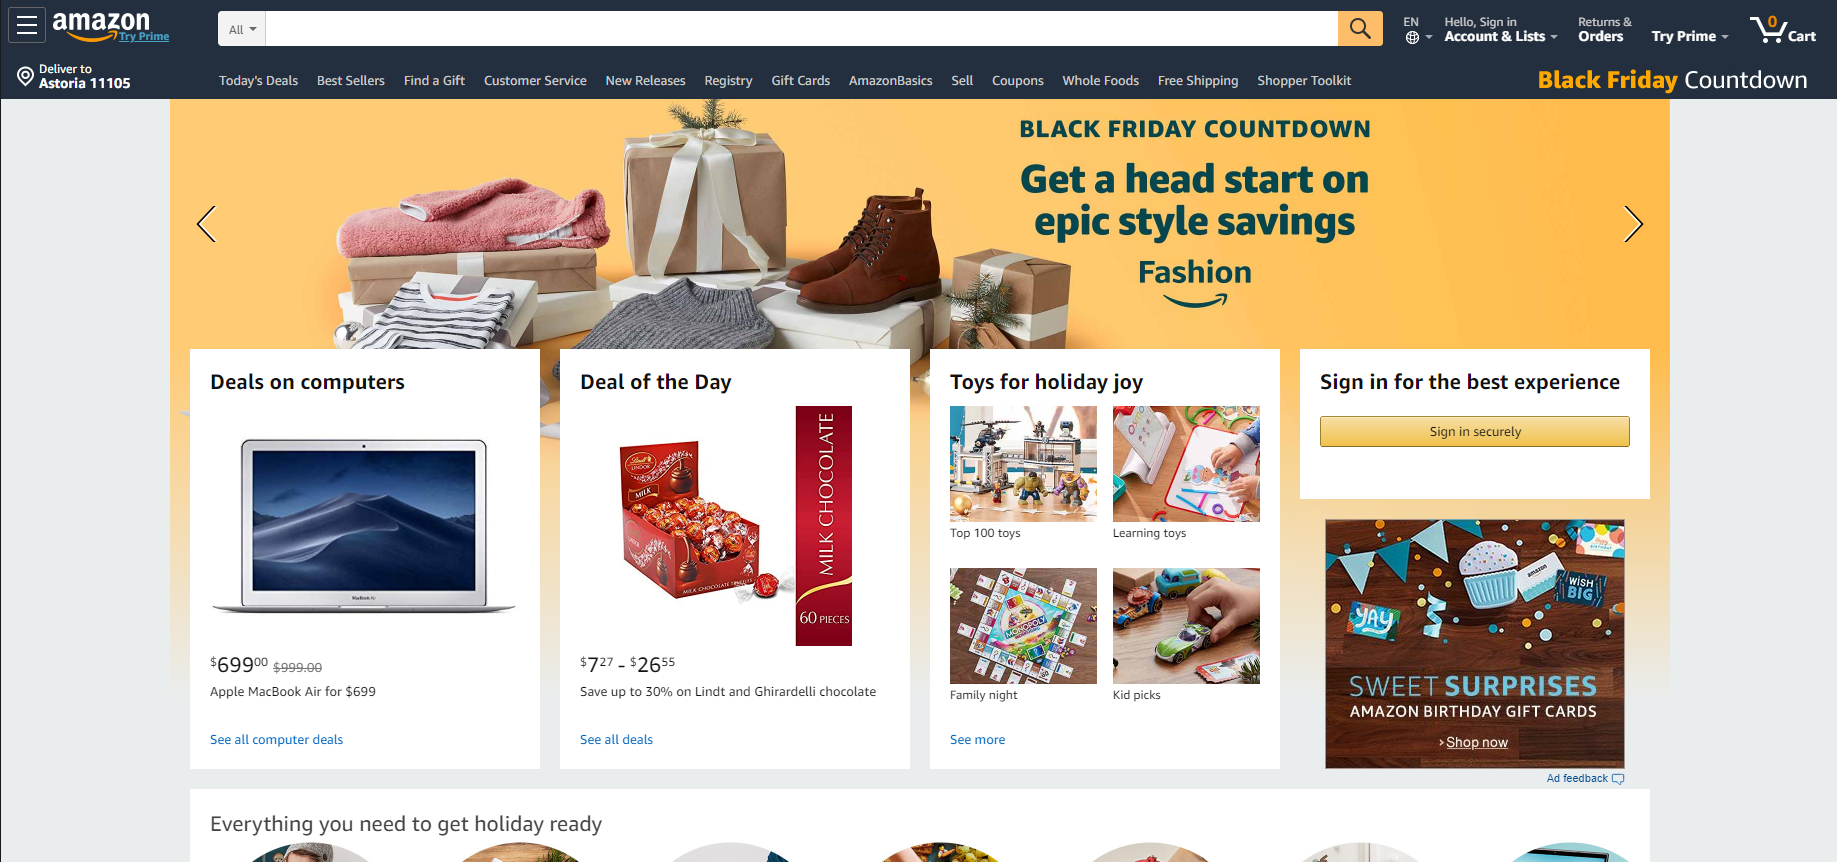
\includegraphics[width=0.8\textwidth]{img/amazon.png}
    \caption{Aplicación \textit{web} dedicada a la venta \textit{on-line}} \label{fig:amazon}
    \end{figure}

    \begin{figure}[H]
    \centering
    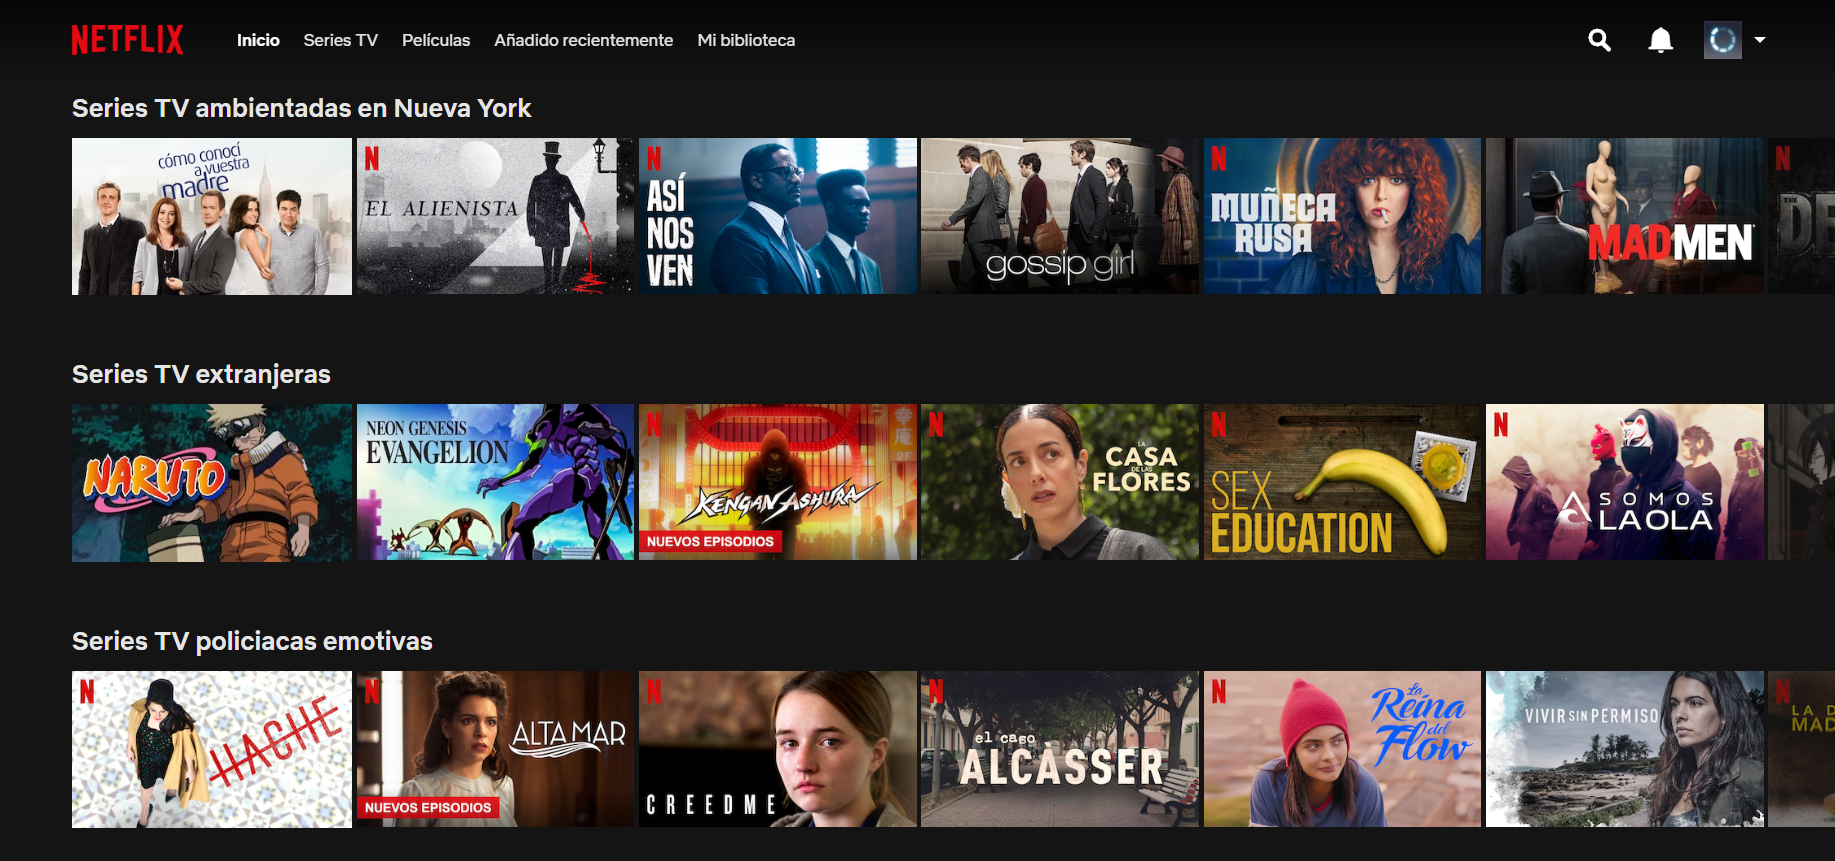
\includegraphics[width=0.8\textwidth]{img/netflix.png}
    \caption{Aplicación \textit{web} dedicada a la distribución de contenidos} \label{fig:netflix}
    \end{figure}
\subsection{HTTP}
\label{subsec:http}
\textit{HiperText Transfer Protocol} (\textit{HTTP}) es el protocolo de nivel de aplicación utilizado para transferir recursos hipermedia entre ordenadores y sigue el esquema petición-respuesta entre cliente y servidor (Figura \ref{fig:http}). En esta comunicación el cliente abre una conexión \textit{TCP} con el servidor y envía un mensaje de petición \textit{HTTP} y, por parte del servidor, responde al cliente con un mensaje \textit{HTTP} y cierra la conexión \textit{TCP}.
El protocolo \textit{HTTP} no mantiene estado. Es decir, el servidor trata cada petición de manera aislada y no almacena información sobre peticiones realizadas por un mismo cliente.
Las peticiones están definidas por el protocolo y tienen métodos concretos:
\begin{itemize}
    \item GET: Solicita un recurso al servidor especificando su \textit{URL}.
    \item HEAD: Método similar a GET con la diferencia de que únicamente solicita las cabeceras y no descarga el recurso completo.
    \item POST: Envía datos al servidor, normalmente un recurso específico que provoca un cambio de estado.
    \item PUT: Actualiza información sobre un recurso del servidor.
    \item DELETE: Elimina en el servidor un recurso.
\end{itemize}

Aunque estos son los principales métodos, el protocolo tiene flexibilidad para ir añadiendo nuevos e incorporar funcionalidad. El número de métodos ha ido aumentando con las nuevas versiones.
\begin{figure}[h]
\centering
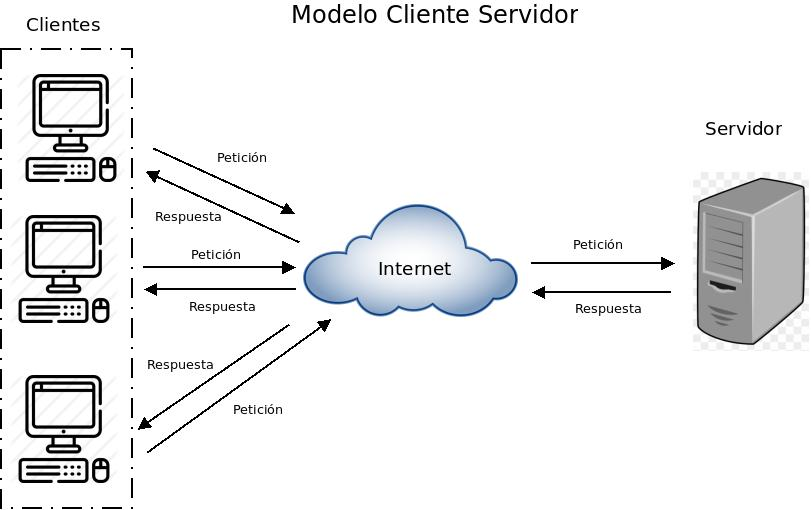
\includegraphics[scale=0.4]{img/http.jpeg}
\caption{Comunicación cliente-servidor en HTTP} \label{fig:http}
\end{figure}

La versión actual del protocolo es del 2 de abril de 2019 (\textit{HTTP/2.4.38}) pero la primera versión es del 1991, que es cuando aparece un estándar para la publicación de páginas web mediante un lenguaje de marcas de hipertexto: \textit{HTML}.


\subsection{Tecnologías en cliente}
\label{subsec:tecclient}
Es la parte encargada de dar forma a la interfaz de usuario y de establecer la comunicación con el servidor. Una pieza importante del cliente es el navegador, ya que es el encargado de leer e interpretar la información recibida. Entre los navegadores \textit{web} más empleados se encuentran \textit{Firefox}, \textit{Google Chrome} u \textit{Opera}\cite{bib:navegadores}. Las tecnologías que hacen posible esa comunicación son:

\begin{itemize}
    \item \textit{\textbf{HTML}}. Estándar más utilizado para el desarrollo de páginas web. Sigue el modelo de objetos \textit{Document Object Model} (\textit{DOM}), que define la manera en la que se comunican dichos objetos con una interfaz para representar documentos. El \textit{DOM} permite el acceso dinámico a través de la programación con lenguajes como \textit{JavaScript} y define como se comunican objetos y elementos con el navegador \textit{web}.
    Actualmente los navegadores usan la versión \textit{HTML5}, que incluye muchas mejoras respecto a su predecesor: \textit{canvas}, \textit{websockets}, \textit{WebRTC}, vídeo, audio, etc. Este lenguaje indica la estructura de una página web, para editar el estilo y presentación visual hay que hacer uso de otros elementos como \textit{CSS}.
    \item \textit{\textbf{Cascading Style Sheets (CSS)}}. Lenguaje de diseño gráfico para definir y crear la presentación de un documento escrito en un lenguaje de marcado. De esta forma, se puede separar información y datos (en los documentos \textit{HTML}) y todo lo relativo al diseño y presentación (en documentos \textit{CSS}). Actualmente los navegadores usan la versión \textit{CSS3}.
    \item \textit{\textbf{JavaScript}}. Lenguaje destinado a programar la lógica, dinamismo e interacción con el usuario. Es el más común y extendido en el desarrollo de páginas. Debido a su importancia en el proyecto, se explicará más a fondo en próximos capítulos.
\end{itemize}

\subsection{Tecnologías en servidor}
\label{subsec:tecserver}
Son las encargadas de dar forma al servidor web de manera que permiten el acceso a herramientas como base de datos, conexiones de red o recursos compartidos. O, dicho de otra forma, se ocupan de realizar las tareas necesarias para hacer posible crear una aplicación que visualizará el cliente. Las más utilizadas son:
\begin{itemize}
    \item \textit{Node.js}: es una forma de ejecutar \textit{JavaScript} en el servidor. Proporciona un entorno de ejecución del lado del servidor que compila y ejecuta a gran velocidad. Esto es debido a que compila en código máquina nativo en lugar de interpretarlo o ejecutarlo.
    \item \textit{Django}: entorno web de alto nivel programado en \textit{python} diseñado para realizar aplicaciones de cualquier complejidad. Es seguro, rápido y escalable. Además, incluye una interfaz para acceder a bases de datos lo que facilita las consultas al no tener que manejar \textit{SQL} y realizarlas con filtros de \textit{Python}.
    \item \textit{Spring}: herramienta basada en \textit{Java} cuya finalidad es simplificar el desarrollo de aplicaciones ya que facilita la configuración de la aplicación y el despliegue en servidor. De esta manera, \textit{Spring} está pensado para aplicaciones web, servicios \textit{REST}, análisis de datos e integración de sistemas.
\end{itemize}

\section{Robótica}
\label{sec:robotica}
La robótica es una rama tecnológica encargada del diseño y construcción de aparatos que realizan operaciones y trabajos en sustitución de la mano de obra humana.

Un robot es un sistema autónomo programable capaz de realizar tareas de ayuda al ser humano y con aplicaciones en campos diversos como la medicina, el hogar, las fábricas, etc.

Los robots se componen de sensores, controladores y actuadores.
\begin{itemize}
    \item \textbf{Sensores}: son los encargados de recoger información del entorno. En este grupo se encuentran lásers, cámaras, ultrasonidos u odómetros. Estos dispositivos equivalen a los sentidos humanos.
    \item \textbf{Controladores}: analizan los datos recogidos por los sensores y elaboran una respuesta que va a ser enviada a los actuadores. En los seres humanos equivale al cerebro.
    \item \textbf{Actuadores}: se encargan de transformar energía eléctrica, hidráulica o neumática en mecánica. Son los que interactúan con el entorno y equivalen a los músculos humanos.
\end{itemize}

\subsection{Aplicaciones robóticas}

La robótica es ya una realidad. Los robots no son utilizados únicamente por empresas para labores industriales, si no que se pueden encontrar en hogares y en la vida cotidiana de las personas. Esto es debido al aumento de eficiencia que generan, reducción de costes o el control de errores que aportan.  Algunas ejemplos de \textit{robots} empleados en la actualidad, tanto en ámbito doméstico como en industrial, son los siguientes:
\begin{itemize}
    \item Aspiradora robótica \textit{Roomba}, robot autónomo que, en los modelos más avanzados, reconocen el entorno, trazan un mapa de la casa y vacían su depósito automáticamente.


    \begin{figure}[H]
\centering

\end{figure}

   \begin{figure}[H]
    \centering
        \begin{subfigure}{0.45\textwidth}           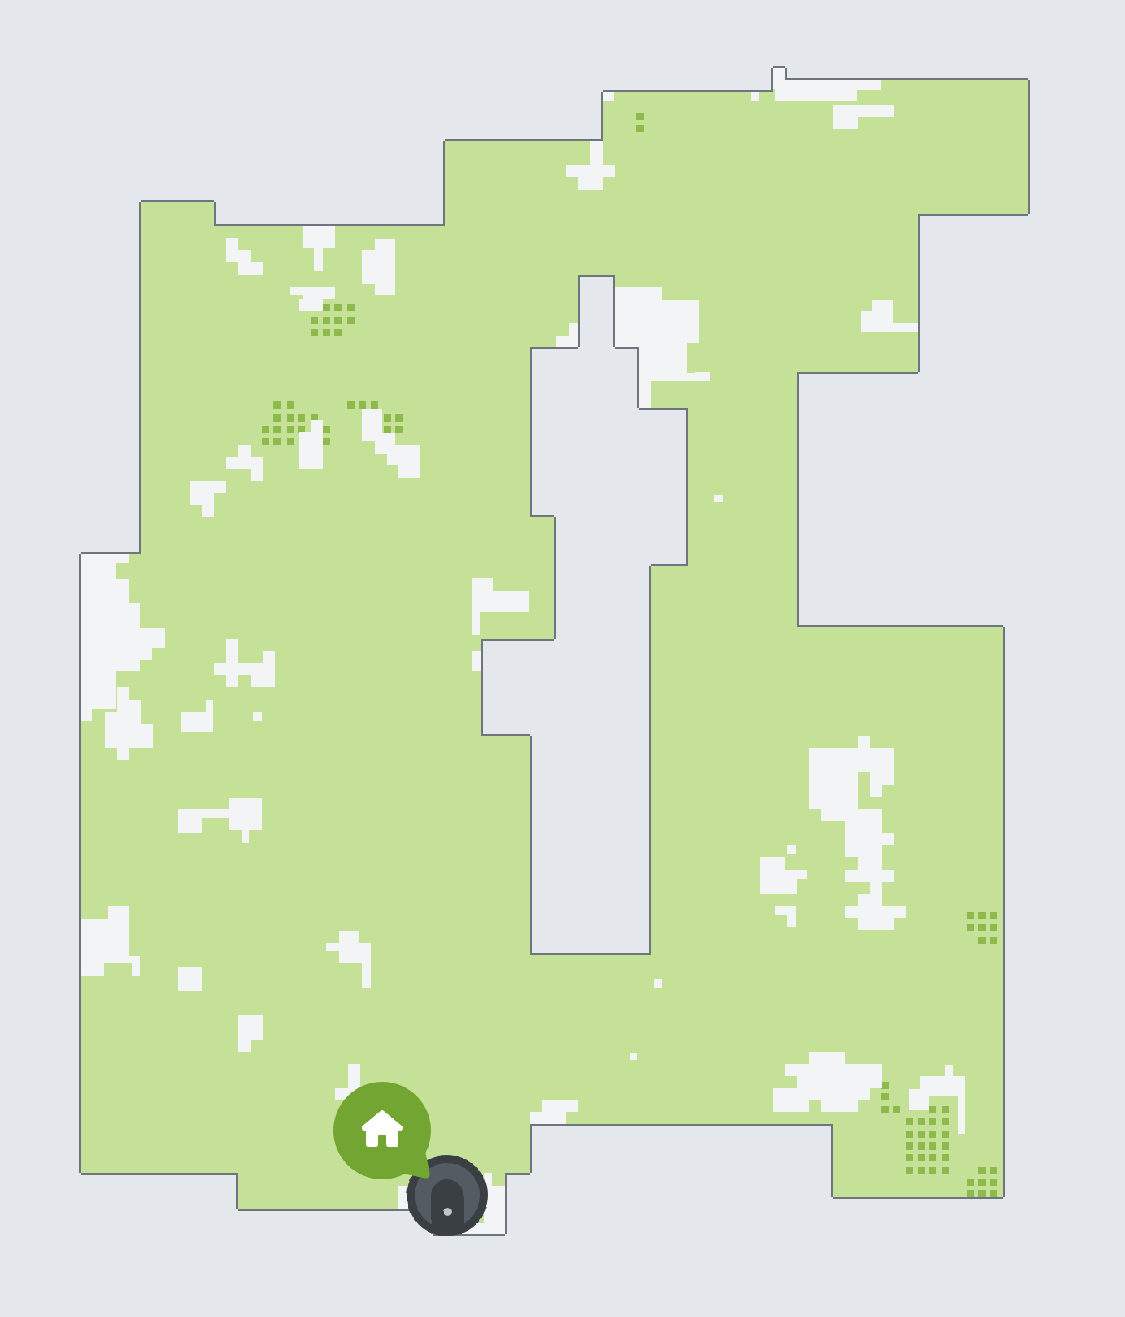
\includegraphics[width=0.8\textwidth]{img/roomba.png}
        \caption{Mapa generado por un robot \textit{Roomba}} \label{fig:roomba}        \label{fig:roombamapa}
        \end{subfigure}
        \begin{subfigure}{0.45\textwidth}
            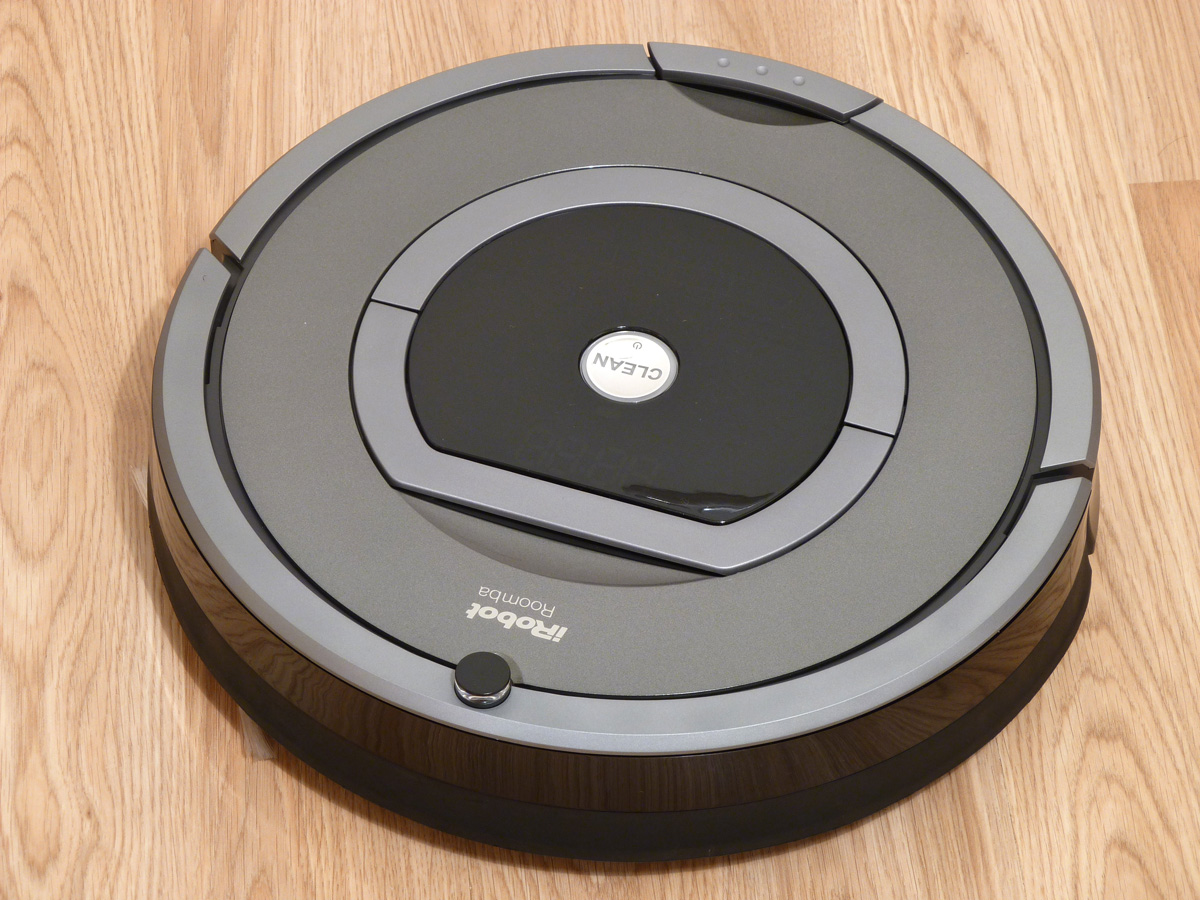
\includegraphics[width=\textwidth]{img/roomba.jpg}
            \caption{Aspirador robótico \textit{Roomba}}
            \label{fig:roombarobot}
        \end{subfigure}
        \label{fig:roomba}
    \end{figure}

    \item Robot médico \textit{Da Vinci}, que permite al cirujano operar a través de una consola mejorando así su precisión y reduciendo riesgos en operaciones quirúrgicas.
      \begin{figure}[H]
    \centering
    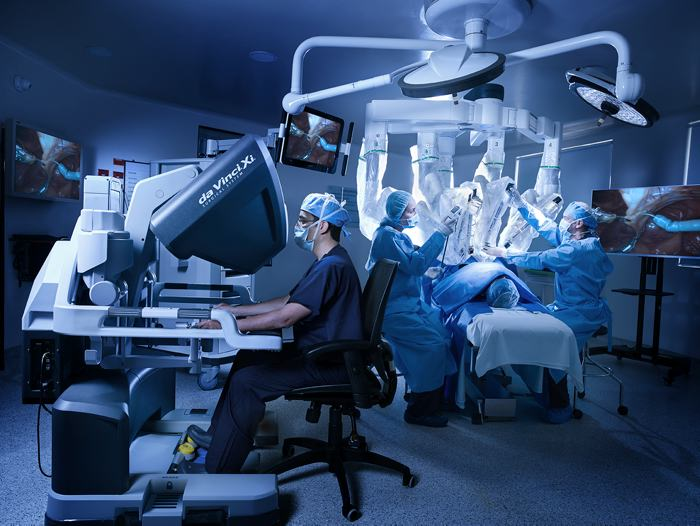
\includegraphics[width=0.6\textwidth]{img/davinci.jpg}
    \caption{Robot médico \textit{Da Vinci}} \label{fig:davinci}
    \end{figure}
    \item Vehículos autónomos \textit{Tesla}, que mediante cámaras y sensores de ultra-sonidos analizan el entorno para garantizar una conducción autónoma segura.


    %   \begin{figure}[H]
    % \centering
    %  \begin{subfigure}{0.6\textwidth}
    %         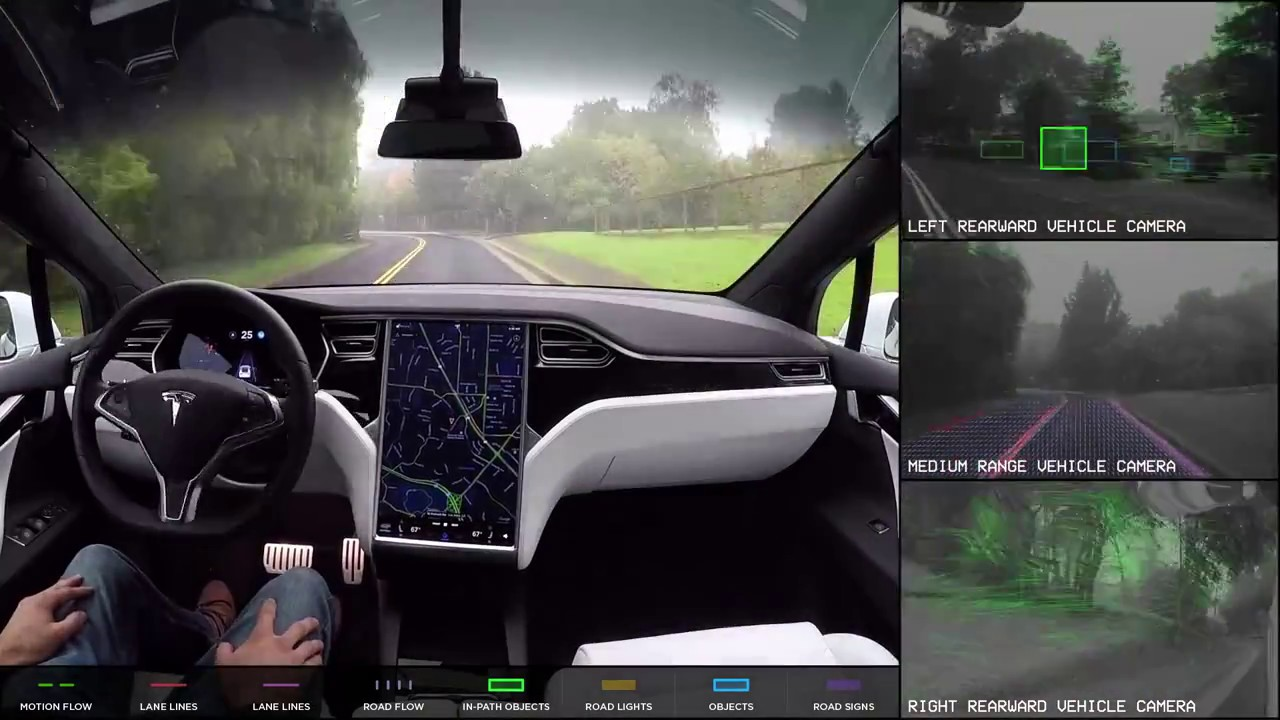
\includegraphics[width=\textwidth]{img/tesla.jpg}
    %         \caption{Coche Tesla con sensores reales}
    %         \label{fig:teslacoche}
    %     \end{subfigure}
    %     \begin{subfigure}{0.35\textwidth}                 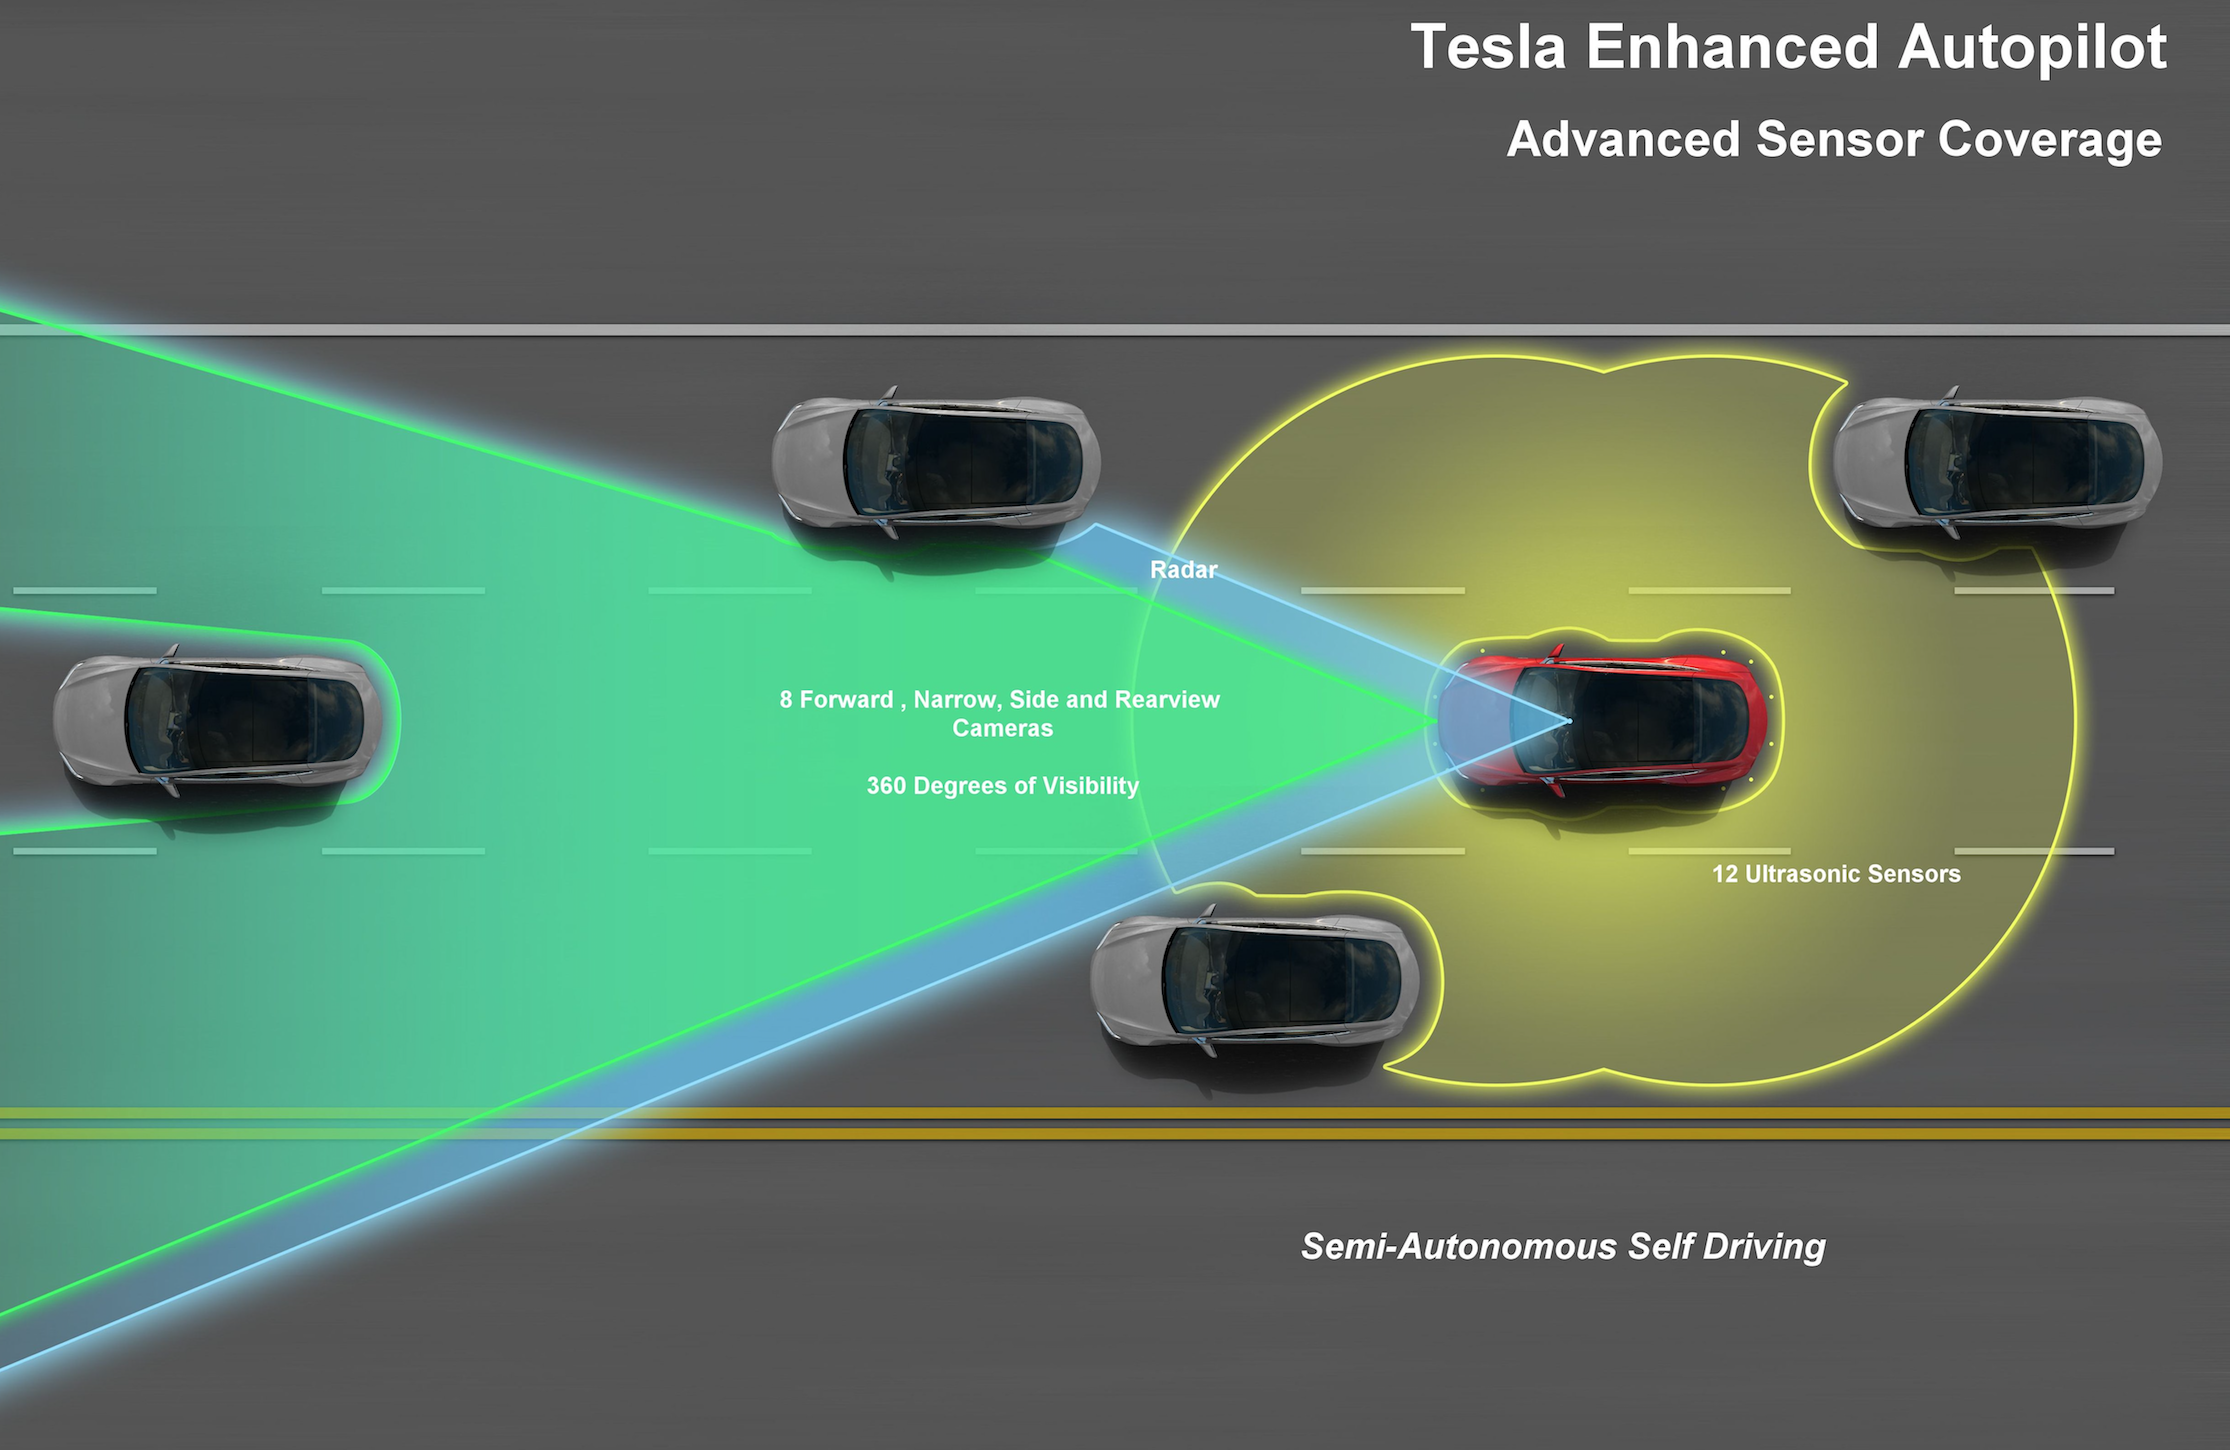
\includegraphics[width=0.9\textwidth]{img/teslaSensors.png}
    %     \caption{Sensores en conducción semi-autónoma} \label{fig:teslasensors}
    %     \end{subfigure}

    %     \label{fig:tesla}
    % \end{figure}

    \begin{figure}[H]
        \centering
        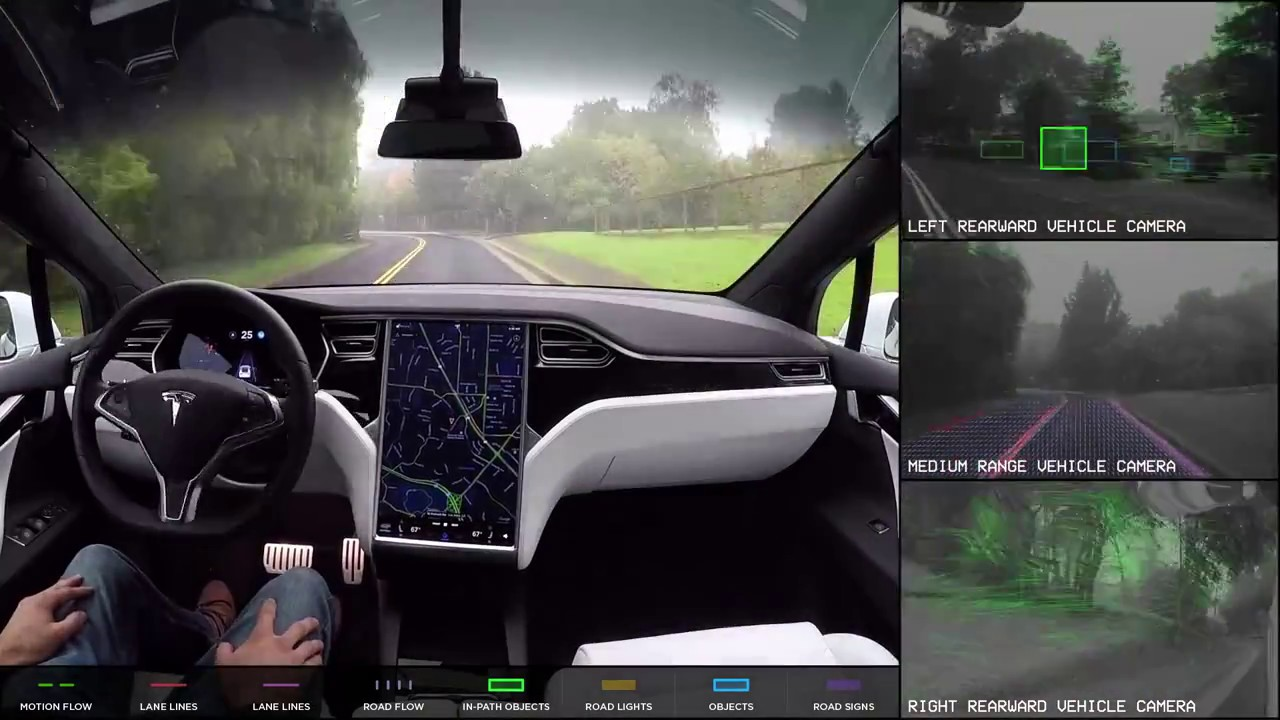
\includegraphics[width=0.7\textwidth]{img/tesla.jpg}
        \caption{Vehículo \textit{Tesla} con imágenes de sus sensores} \label{fig:tesla}
    \end{figure}

    \item Robots de logística de \textit{Amazon}, que se encargan, de manera autónoma, de localizar la estantería donde se encuentra un paquete solicitado y la desplaza por todo el centro logístico al lugar de destino.
        \begin{figure}[H]
    \centering
    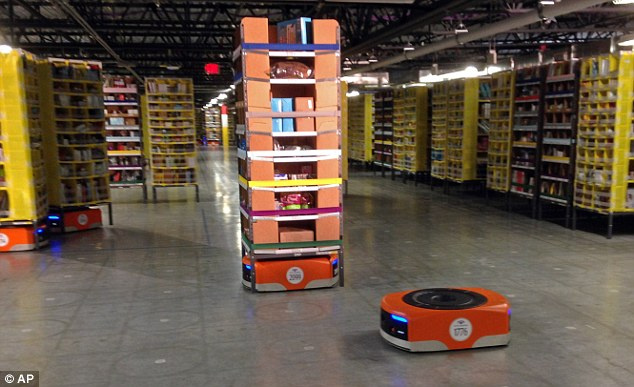
\includegraphics[width=0.65\textwidth]{img/robots-amazon.jpg}
    \caption{Robots de logística de \textit{Amazon}} \label{fig:amazon}
    \end{figure}
    \item Robot \textit{Curiosity} de la \textit{NASA}, empleado para la exploración de la superficie del planeta Marte.
    \begin{figure}[H]
    \centering
    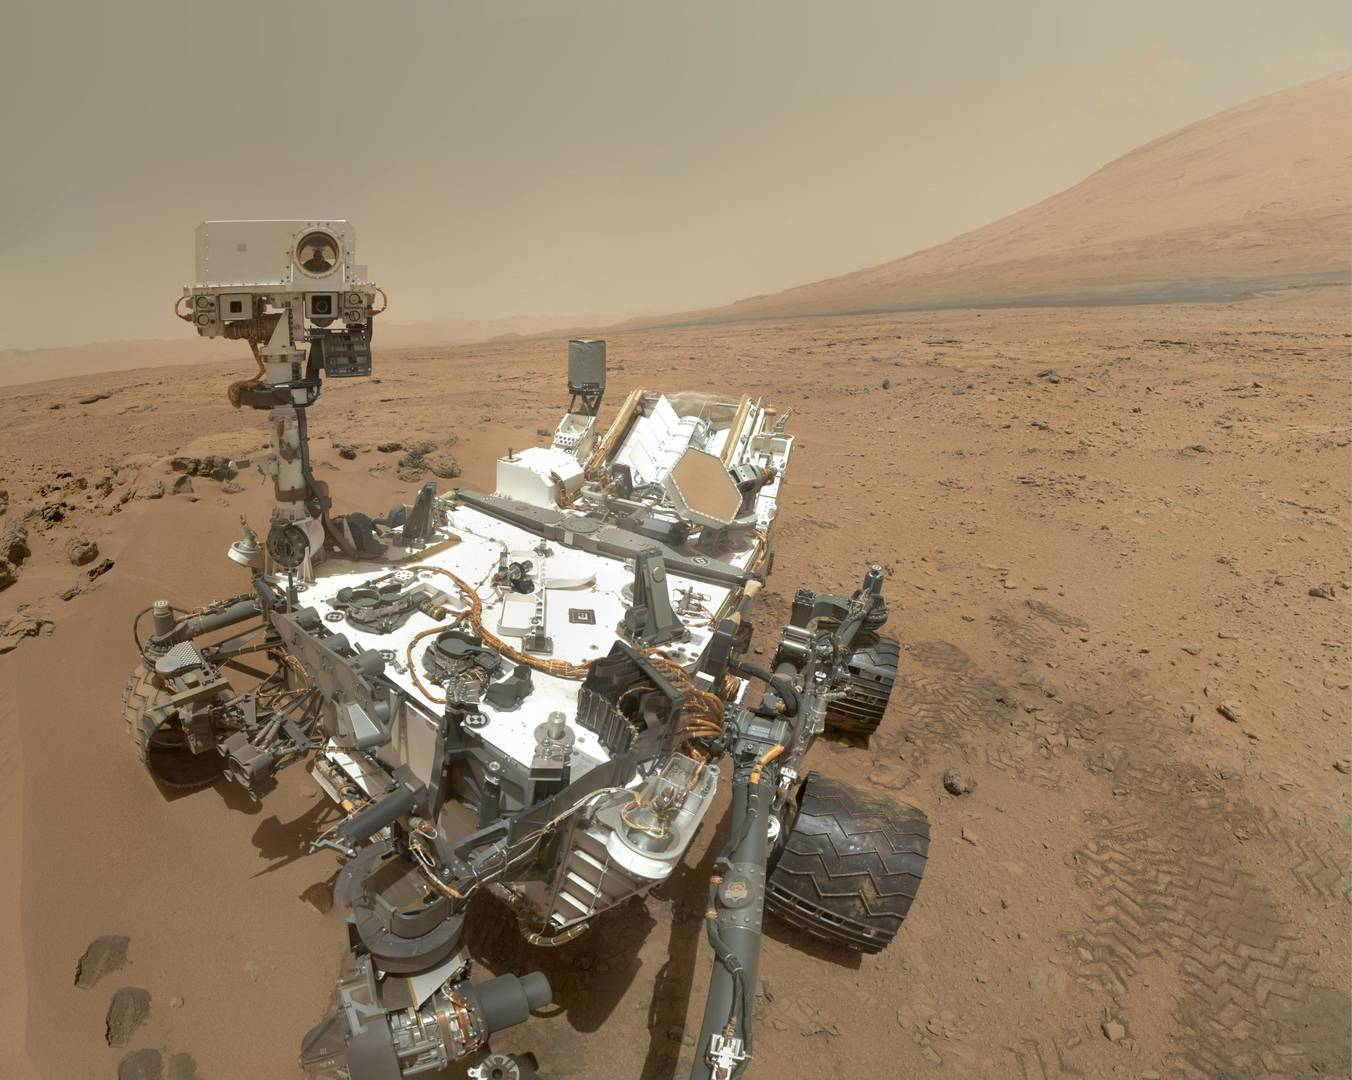
\includegraphics[width=0.5\textwidth]{img/curiosity.jpg}
    \caption{Robot \textit{Curiosity} de la \textit{NASA}} \label{fig:curiosity}
    \end{figure}
\end{itemize}{}

\subsection{Software en robótica}
\label{subsec:softwarerobot}
Para dotar de inteligencia autónoma a los robots se requiere desarrollar sistemas  complejos, aplicaciones e infraestructuras. Por ejemplo, hace años, el desarrollo de \textit{software} se realizaba adoptando soluciones ``\textit{ad-hoc}'' dotando a cada robot de un diseño específico y con sensores y actuadores concretos. Esto implicaba que había que implementar todo el \textit{software} para un nuevo robot debido a que no se podía aplicar el desarrollado anteriormente. En la actualidad, existen plataformas que permiten el desarrollo de aplicaciones robóticas de forma eficiente y genérica permitiendo así reutilizar aplicaciones creadas en otros robots. \\


Para dotar de inteligencia a un robot se desarrolla un \textit{software} que habitualmente se programa con ayuda de herramientas, como los \textit{middleware} robóticos. El uso de estas herramientas permiten introducir una capa de abstracción con los \textit{drivers} y el \textit{hardware} del robot, reduciendo la complejidad y los conocimientos necesarios para realizar desarrollos. Algunas de estos \textit{middleware} son:
\begin{itemize}
    \item \textit{\textbf{Robot Operating System (ROS)}}\cite{bib:ros}. Plataforma de \textit{software} libre para el desarrollo de \textit{software} de robots. Provee servicios estándar de un sistema operativo como la abstracción de \textit{hardware}, control de dispositivos de bajo nivel, mecanismos de intercambio de mensajes entre procesos y una serie de herramientas utilizadas en robótica.
    \item \textit{\textbf{ORCA}}\cite{bib:orca}. Plataforma de \textit{software} libre dedicada al desarrollo de aplicaciones robóticas. Dedicada principalmente al desarrollo de componentes, que se pueden ejecutar de manera independiente o se pueden unir para formar sistemas robóticos de distintas complejidades. Permite reutilizar código y emplear componentes robóticos ya creados.
     \item \textit{\textbf{OROCOS}}\cite{bib:orocos} Proyecto de \textit{software} libre dedicado al control de robots y máquinas. Está orientado a componentes y permite añadir funcionalidad de manera sencilla y sin recopilar todo el código. Incluye paquetes complementarios como filtros de \textit{Bayes}, librerías de control dinámico y cinemático o visión.
\end{itemize}

\section{Robótica educativa}
\label{sec:educativa}
La robótica con fines educativos está empezando a adquirir importancia en la enseñanza porque su aprendizaje está disponible para estudiantes de cualquier nivel. Este método de enseñanza intenta despertar el interés de los alumnos porque, gracias a la innovación que posibilita la tecnología, añade un componente atractivo e integrador a las asignaturas tradicionales. En 2015 la comunidad de Madrid introdujo la asignatura de robótica en los planes docentes de Enseñanza Secundaria con la asignatura ``Tecnología, Programación y Robótica''\cite{bib:secundaria} y en el curso 2020-2021 se empezará a implantar en Educación Primaria la asignatura ``Programación y Robótica''\cite{bib:primaria}.\\

El método más empleado para este tipo de enseñanza es la educación \textit{STEM} (\textit{Science, Technology, Engineering and Mathematics}). Este tipo de educación promueve una cultura de pensamiento científico, así como la adquisición de conocimientos tecnológicos aplicables a situaciones reales y permite desarrollar competencias para la resolución de problemas y un pensamiento creativo y crítico.   \\


La enseñanza en centros escolares se realiza en gran parte mediante plataformas como la creada por LEGO o placas Arduino que simplifican el aprendizaje y resulta motivadora para el alumno porque obtiene resultados vistosos y se le puede dar una aplicación real. \\

Resulta importante acercar la robótica a alumnos en edades muy tempranas, partiendo de nociones básicas, dada la importancia que está adquiriendo la disciplina y la fuerte presencia que tiene en la mayor parte de los sectores laborales. Además, la capacidad de programar es una parte importante en la sociedad actual ya que, con esta habilidad, se aprenden estrategias para resolver problemas, diseñar proyectos y comunicar ideas. \\


Una manera de acercar estas nociones básicas son los lenguajes de programación visual. Se trata de lenguajes potentes y muy intuitivos que abstraen al alumno de la complejidad que implica la sintaxis y aportan un entorno visual haciendo que el software sea bien aceptado por estudiantes de corta edad. Además permiten a los usuarios programar manipulando elementos gráficos en lugar de hacerlo textualmente. Los lenguajes de programación visual más importantes son:

\begin{itemize}
    \item \textit{\textbf{Scratch}}\cite{bib:scratch}: proyecto liderado por el \textit{MIT}, es utilizado por estudiantes y docentes para programar animaciones, juegos e interacciones fácilmente gracias a su interfaz visual. Se trata de un lenguaje donde los programas se construyen ensamblando bloques gráficos y cada bloque es el equivalente a una función o método de cualquier lenguaje de programación. Actualmente está en su versión \textit{Scratch 3.0} y en la figura \ref{fig:scratch} se puede ver un ejemplo de su interfaz gráfica.
    \begin{figure}[H]
    \centering
    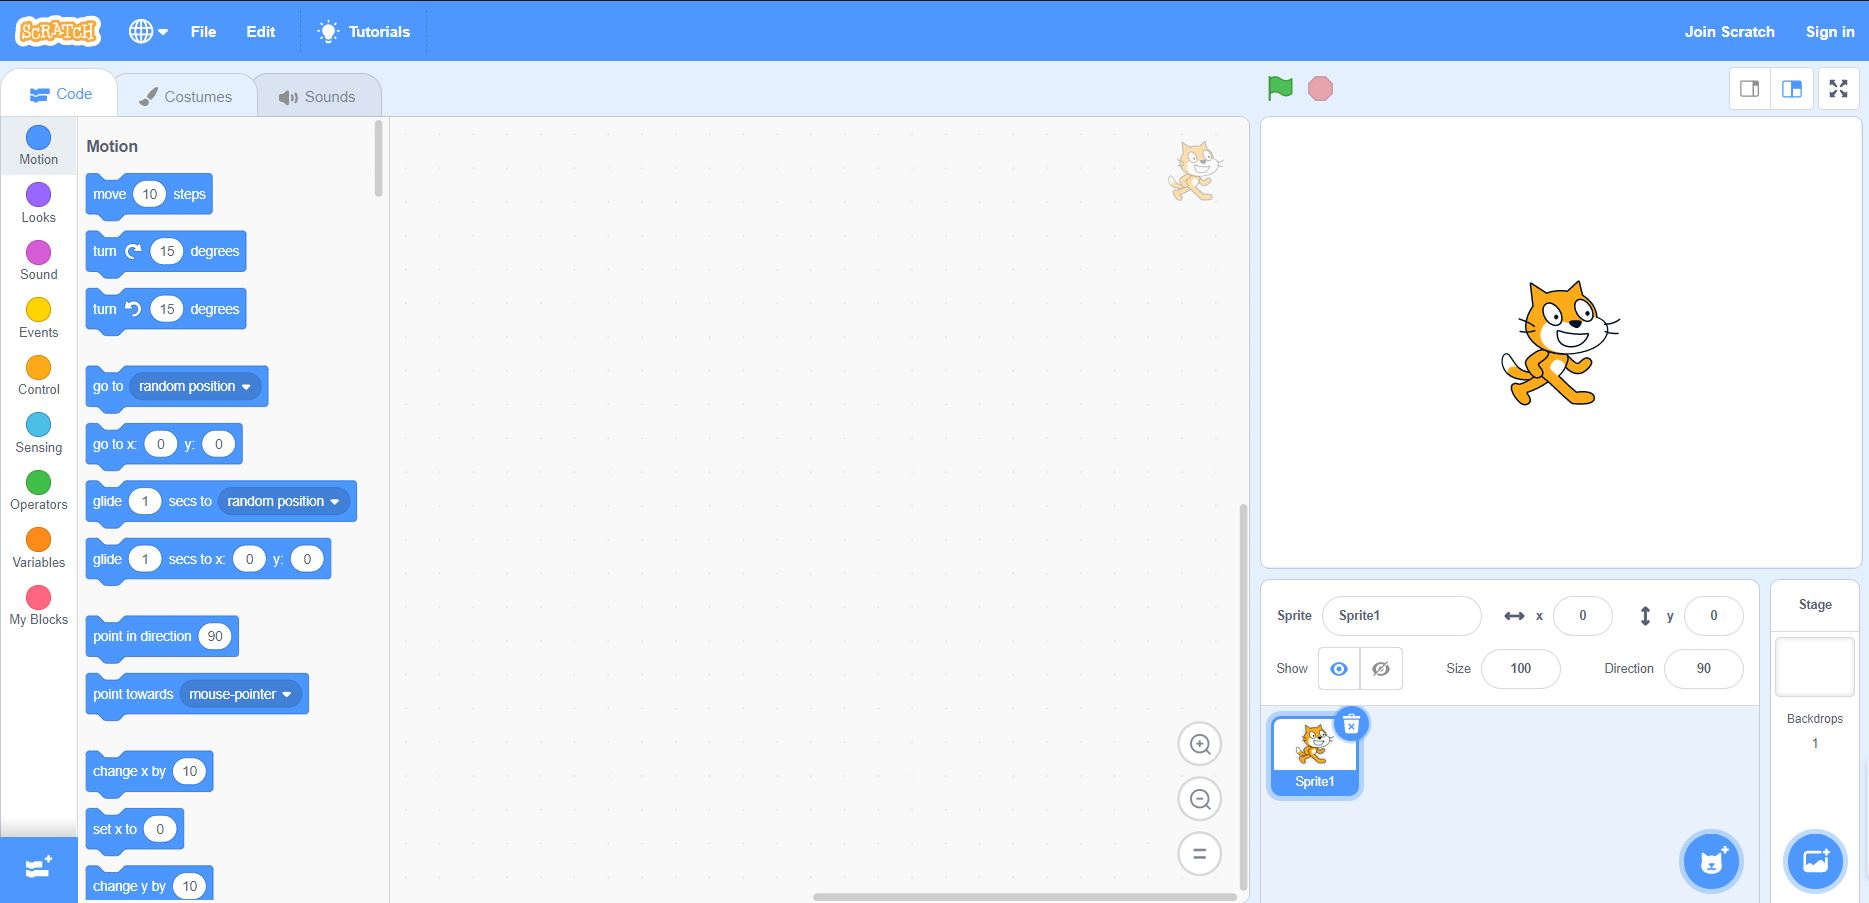
\includegraphics[width=0.7\textwidth]{img/scratch.jpg}
    \caption{Interfaz gráfica de Scratch} \label{fig:scratch}
    \end{figure}

    \item \textit{\textbf{LEGO}}\cite{bib:lego}: dispone de una amplia gama de robots programables y cada uno de ellos tiene un sistema gráfico. En la figura \ref{fig:lego} se pueden ver dos ejemplos de distintos software para distintos robots.

    \begin{figure}[H]
    \centering
        \begin{subfigure}{0.45\textwidth}           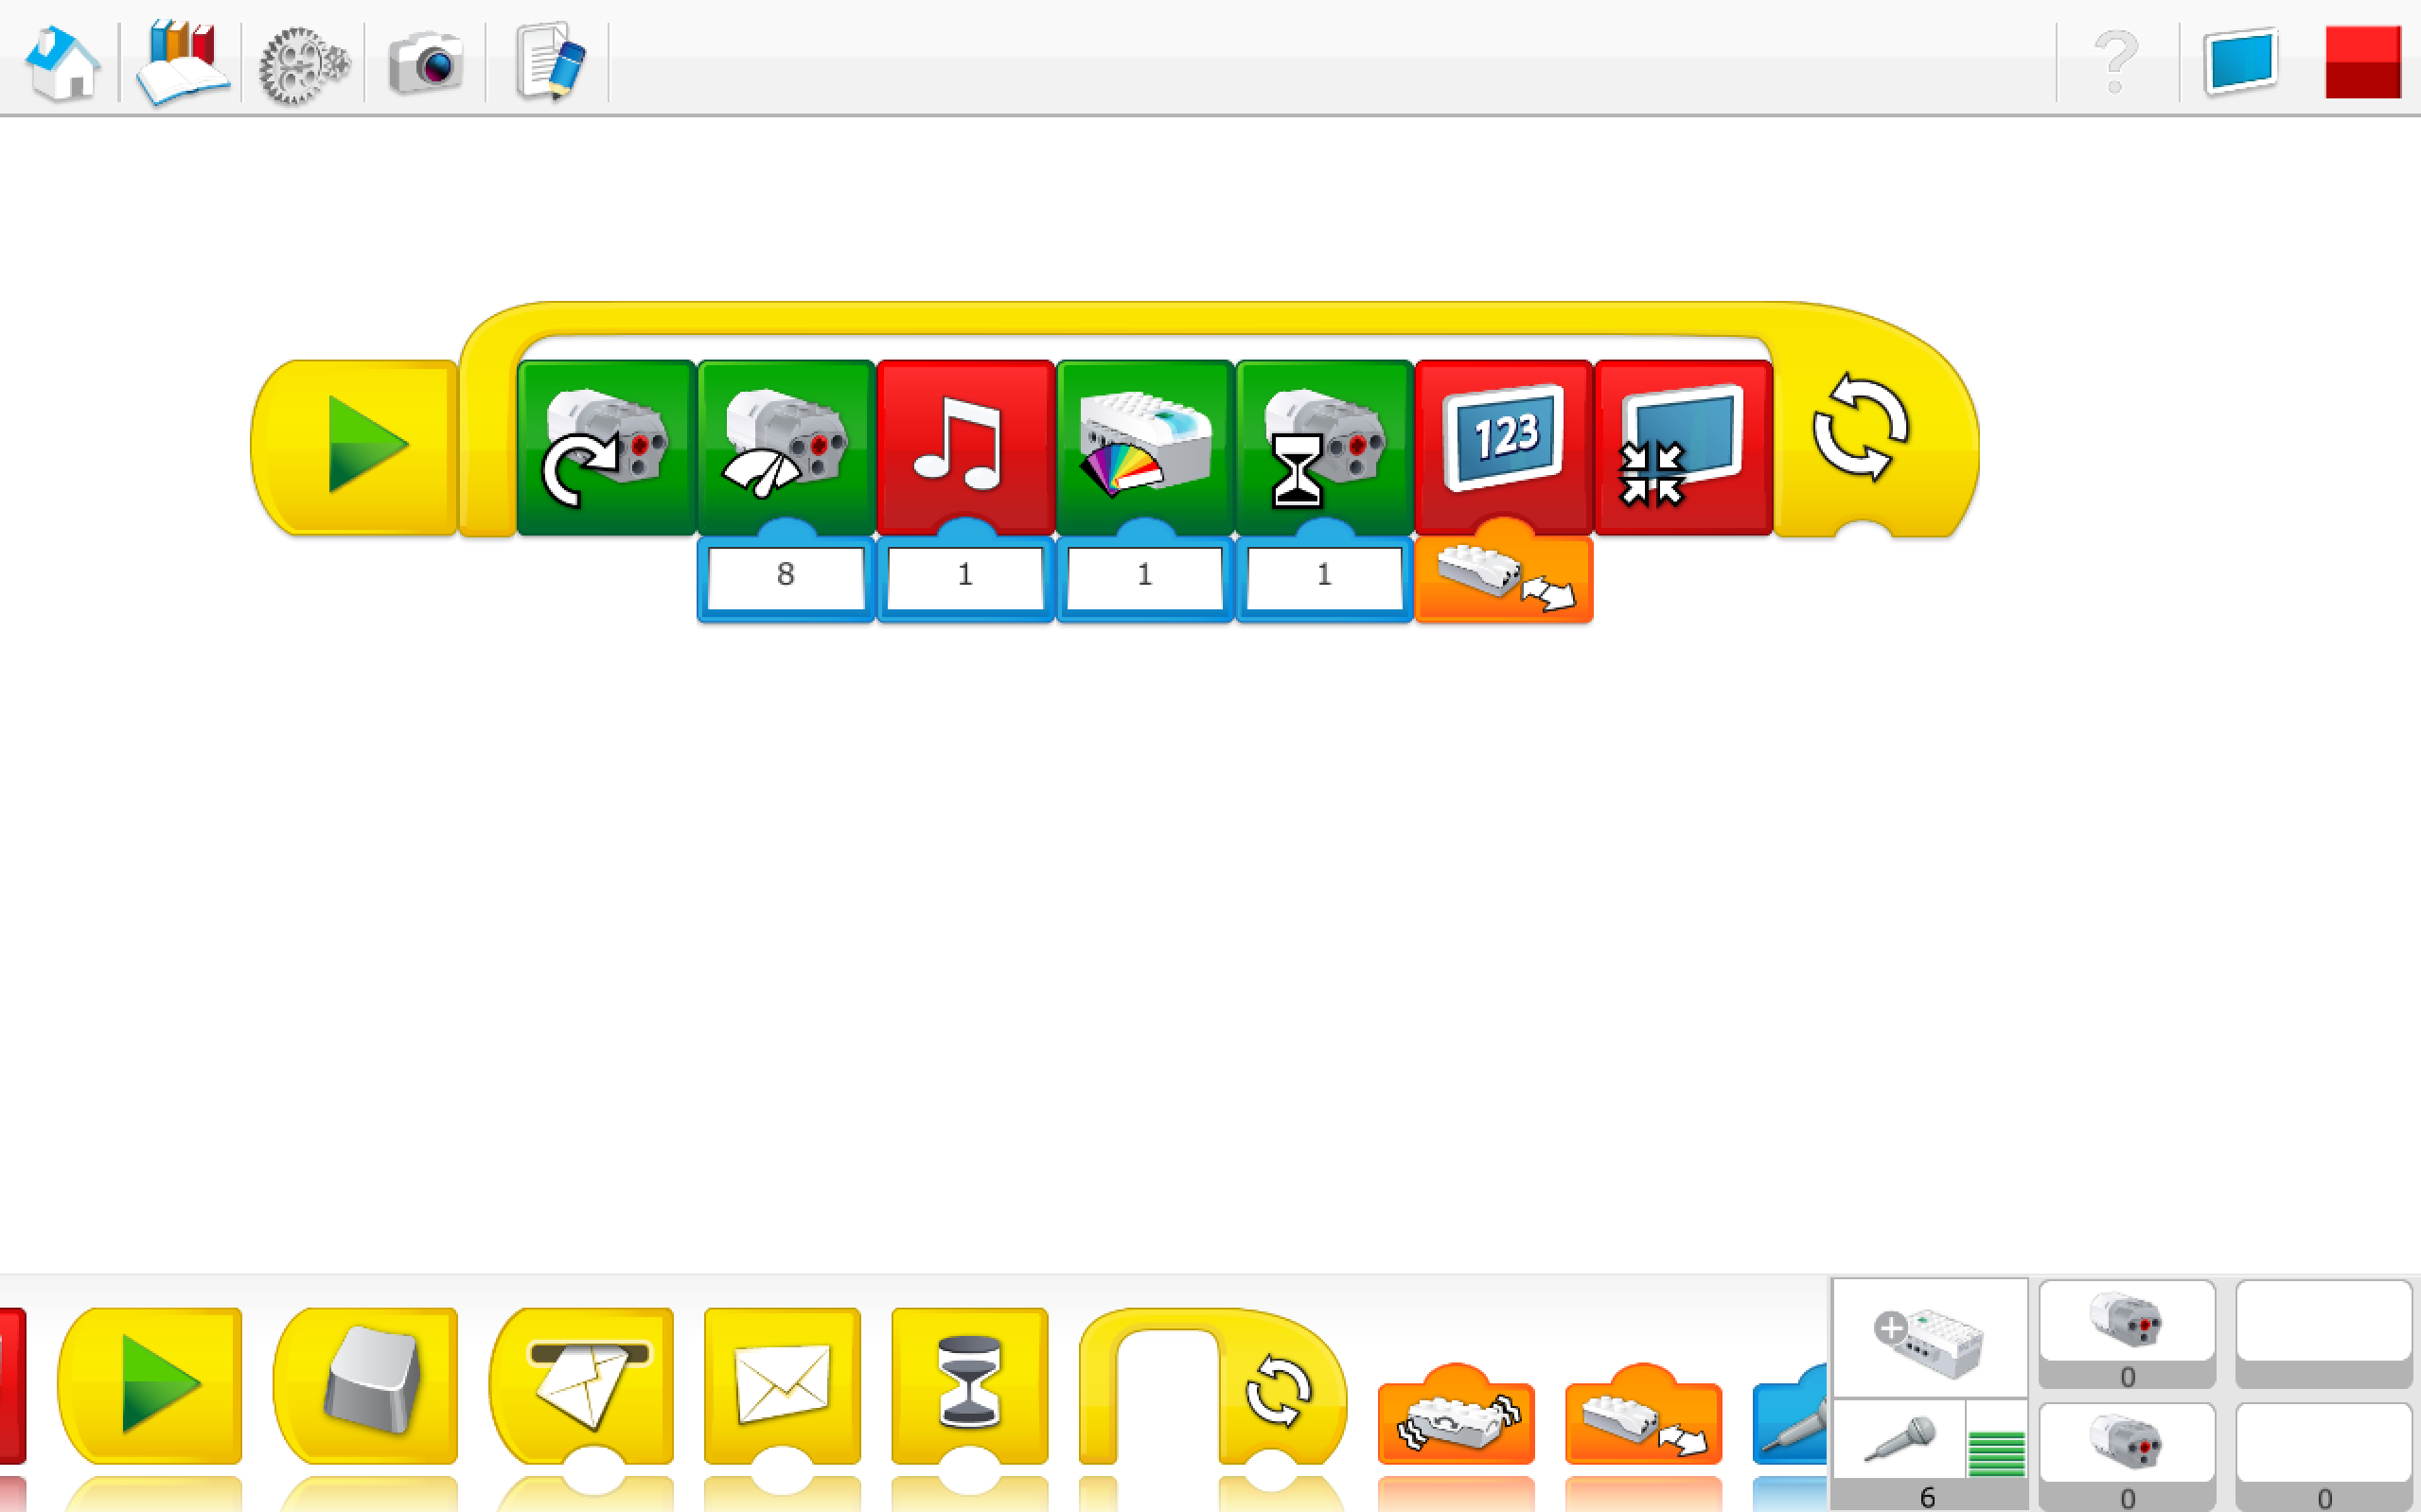
\includegraphics[width=\textwidth]{img/lego1.png}
           \caption{Interfaz gráfica de LEGO WeDo 2.0}             \label{fig:lego1}
        \end{subfigure}
        \begin{subfigure}{0.45\textwidth}
            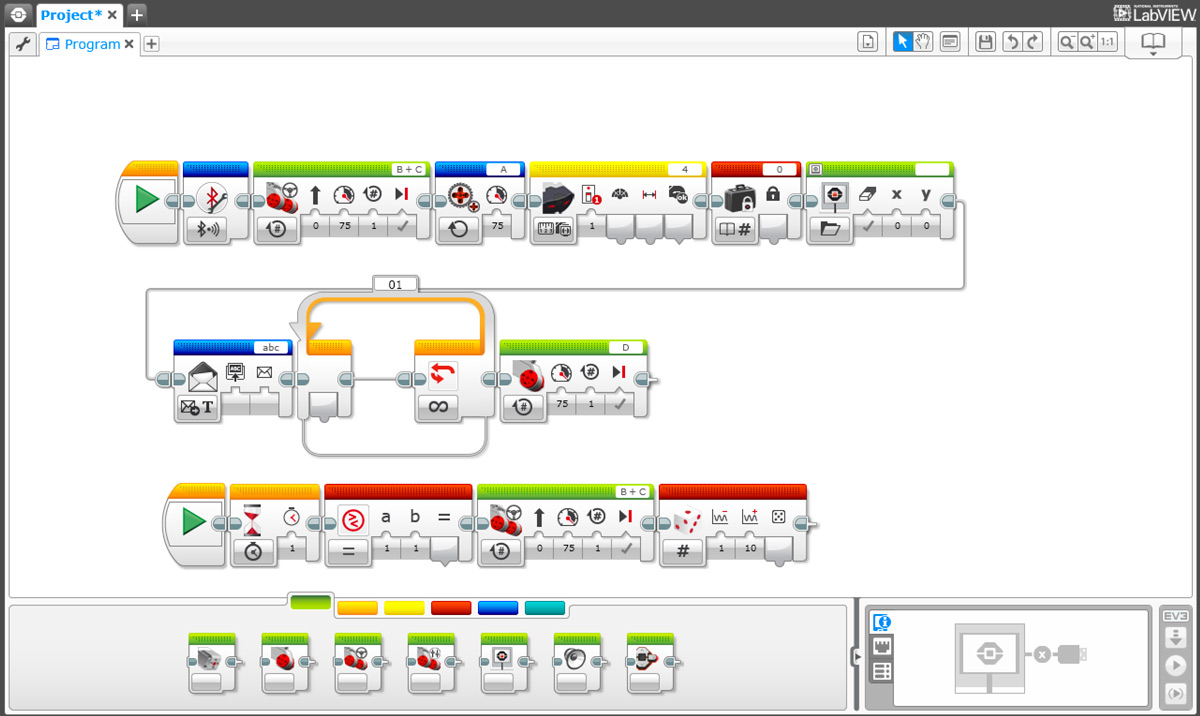
\includegraphics[width=\textwidth]{img/lego2.jpg}
            \caption{Interfaz gráfica de LEGO MINDSTORMS EV3}
            \label{fig:lego2}
        \end{subfigure}
        \label{fig:lego}
    \end{figure}

    \item \textit{\textbf{Kodu}}\cite{bib:kodu}: lenguaje de programación visual creado por Microsoft para desarrollar videojuegos. Diseñado para ser muy accesible y agradable para cualquier usuario siendo un lenguaje basado en reglas, condiciones y acciones prescindiendo de muchas convecciones de programación como bucles, subrutinas o variables simbólicas. Permite a los más jóvenes ser creadores de sus propios videojuegos.

    \begin{figure}[H]
        \centering
        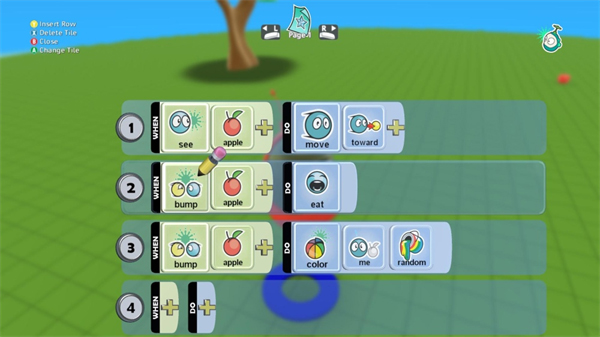
\includegraphics[width=0.9\textwidth]{img/kodu.jpg}
        \caption{Interfaz gráfica de Kodu} \label{fig:kodu}
    \end{figure}

    \item \textit{\textbf{Snap!}}\cite{bib:snap}: basado en \textit{Scratch}, sigue su facilidad para aprender a programar pero su uso se concentra en edades algo más avanzadas. Accesible desde cualquier navegador al estar programado en \textit{JavaScript}.

    \begin{figure}[H]
        \centering
        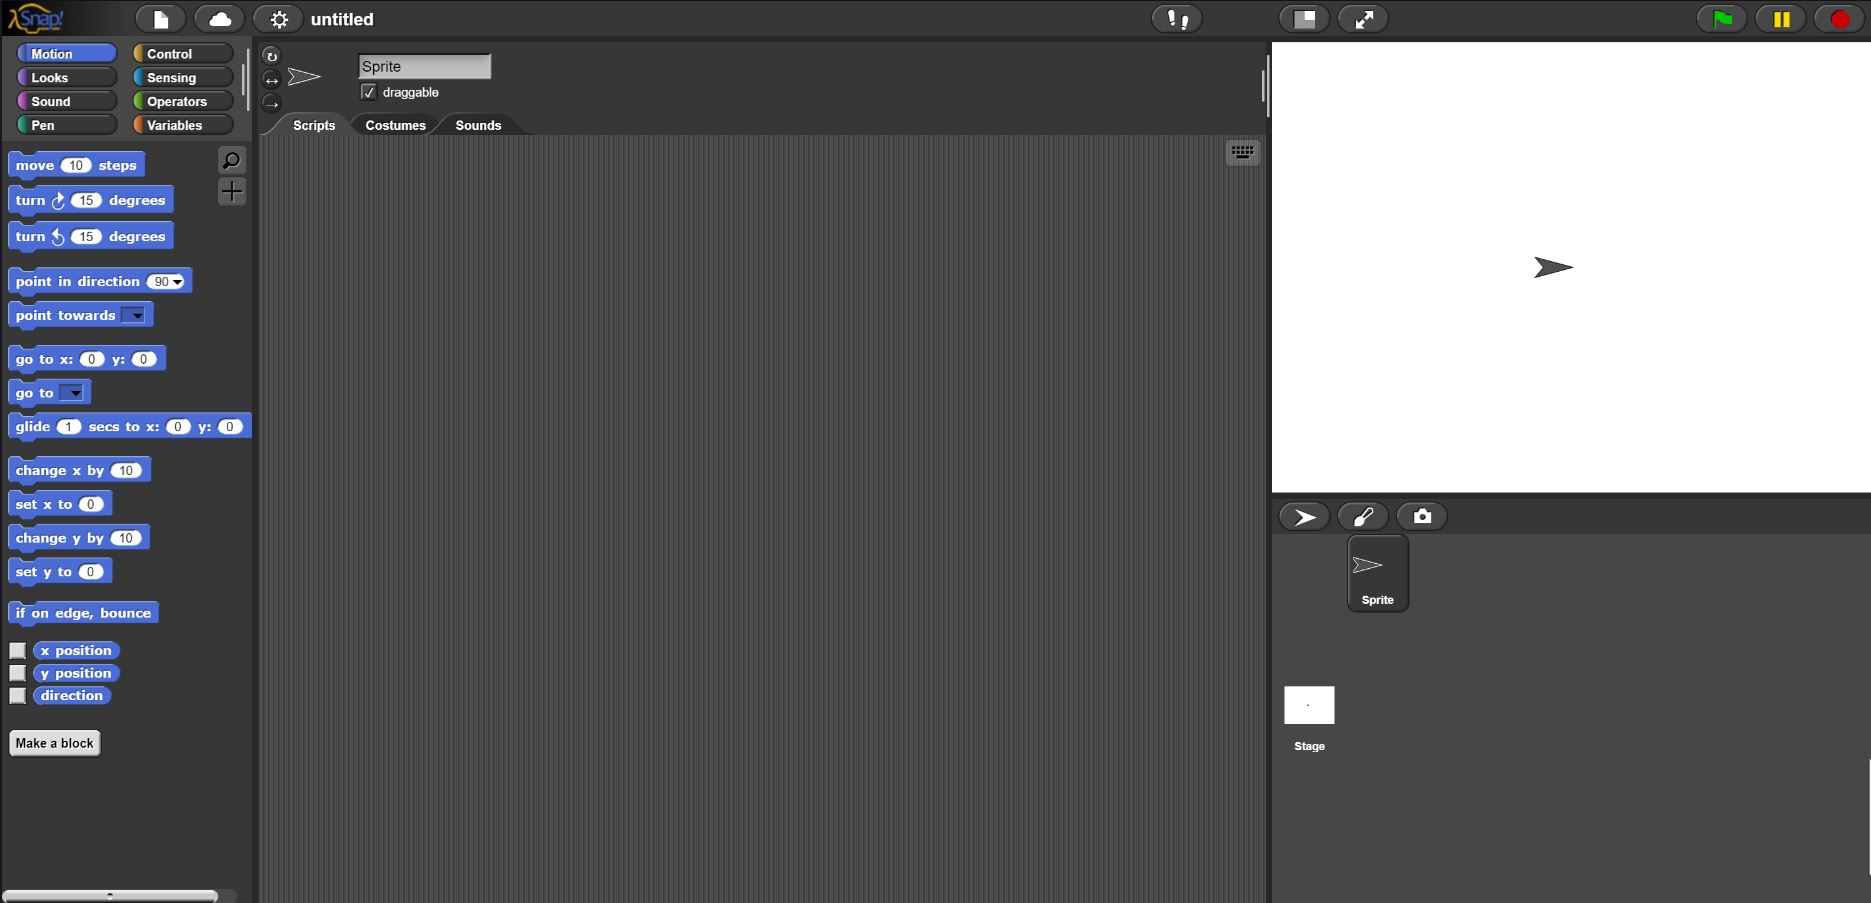
\includegraphics[width=0.9\textwidth]{img/snap.jpg}
        \caption{Interfaz gráfica de Snap!} \label{fig:snap}
    \end{figure}

    \item \textit{\textbf{AppInventor}}\cite{bib:appinventor}: Entorno de desarrollo de software creado por \textit{Google} en colaboración con el \textit{MIT} destinado a la elaboración de aplicaciones \textit{Android}. El usuario puede desarrollar de forma visual y con ayuda de bloques una aplicación que cubre un gran número de necesidades básicas en un dispositivo móvil.
        \begin{figure}[h]
        \centering
        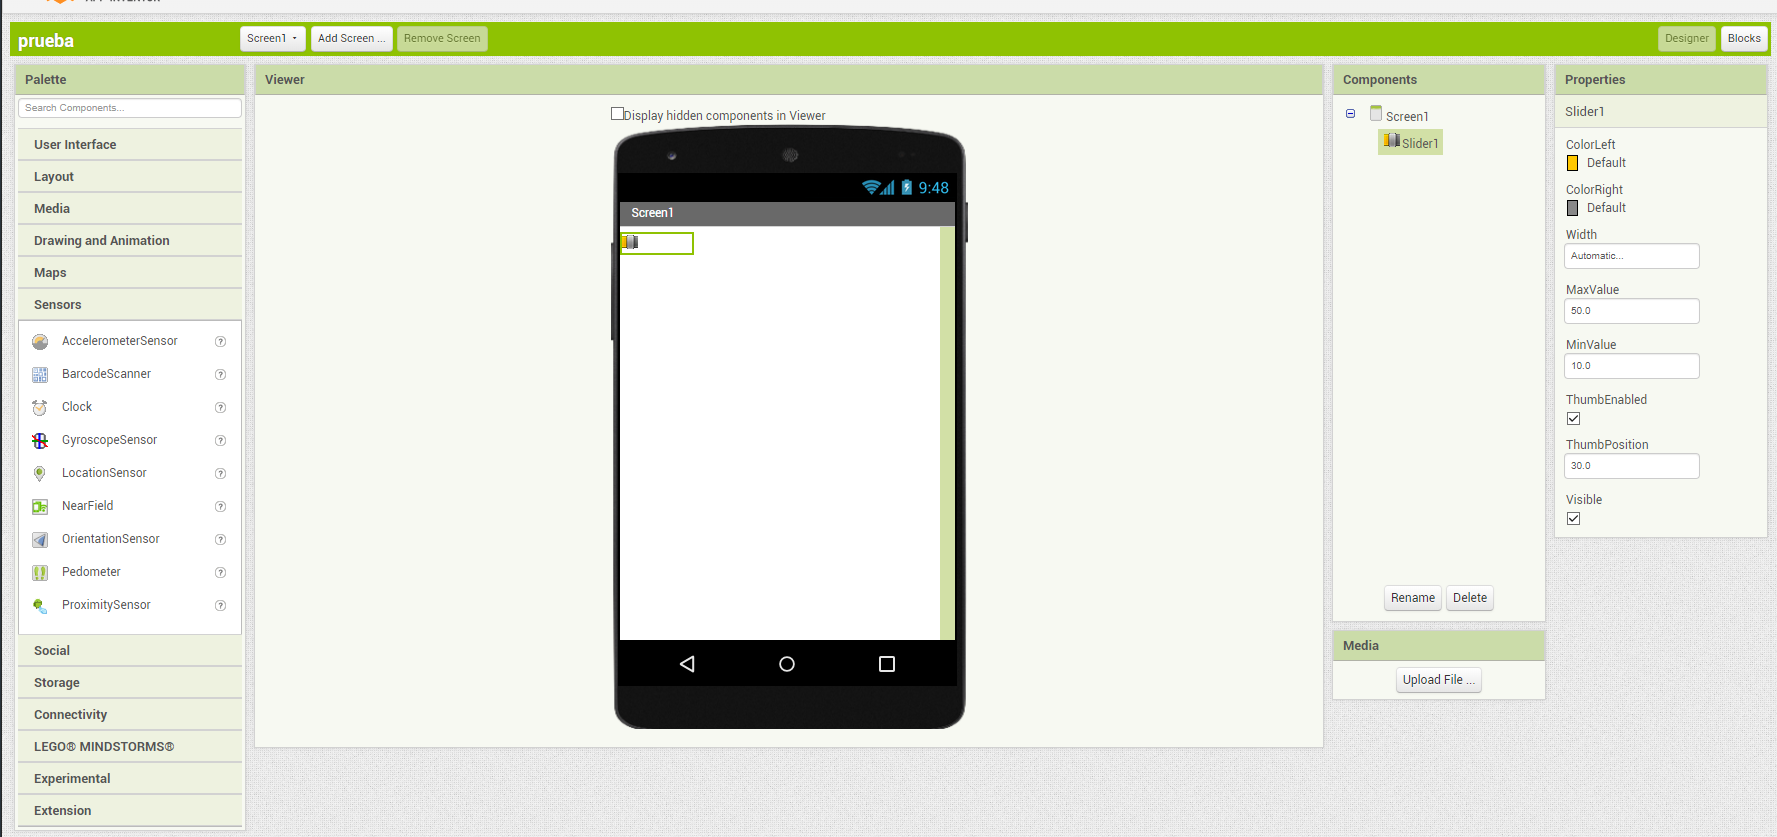
\includegraphics[width=0.9\textwidth]{img/AppInventor.png}
        \caption{Interfaz gráfica de AppInventor} \label{fig:appinventor}
    \end{figure}

\end{itemize}


También es habitual en robótica educativa el uso de plataformas hardware, que incorporan los elementos básicos para la construcción de un robot. Las más empleadas son:
\begin{itemize}
    \item \textit{\textbf{LEGO mindstorms}}: plataforma dedicada a construir \textit{robots} con piezas de LEGO. También incluye un microprocesador para ser programado, sensores (infrarrojos, táctiles y de color) y motores.
            \begin{figure}[H]
        \centering
        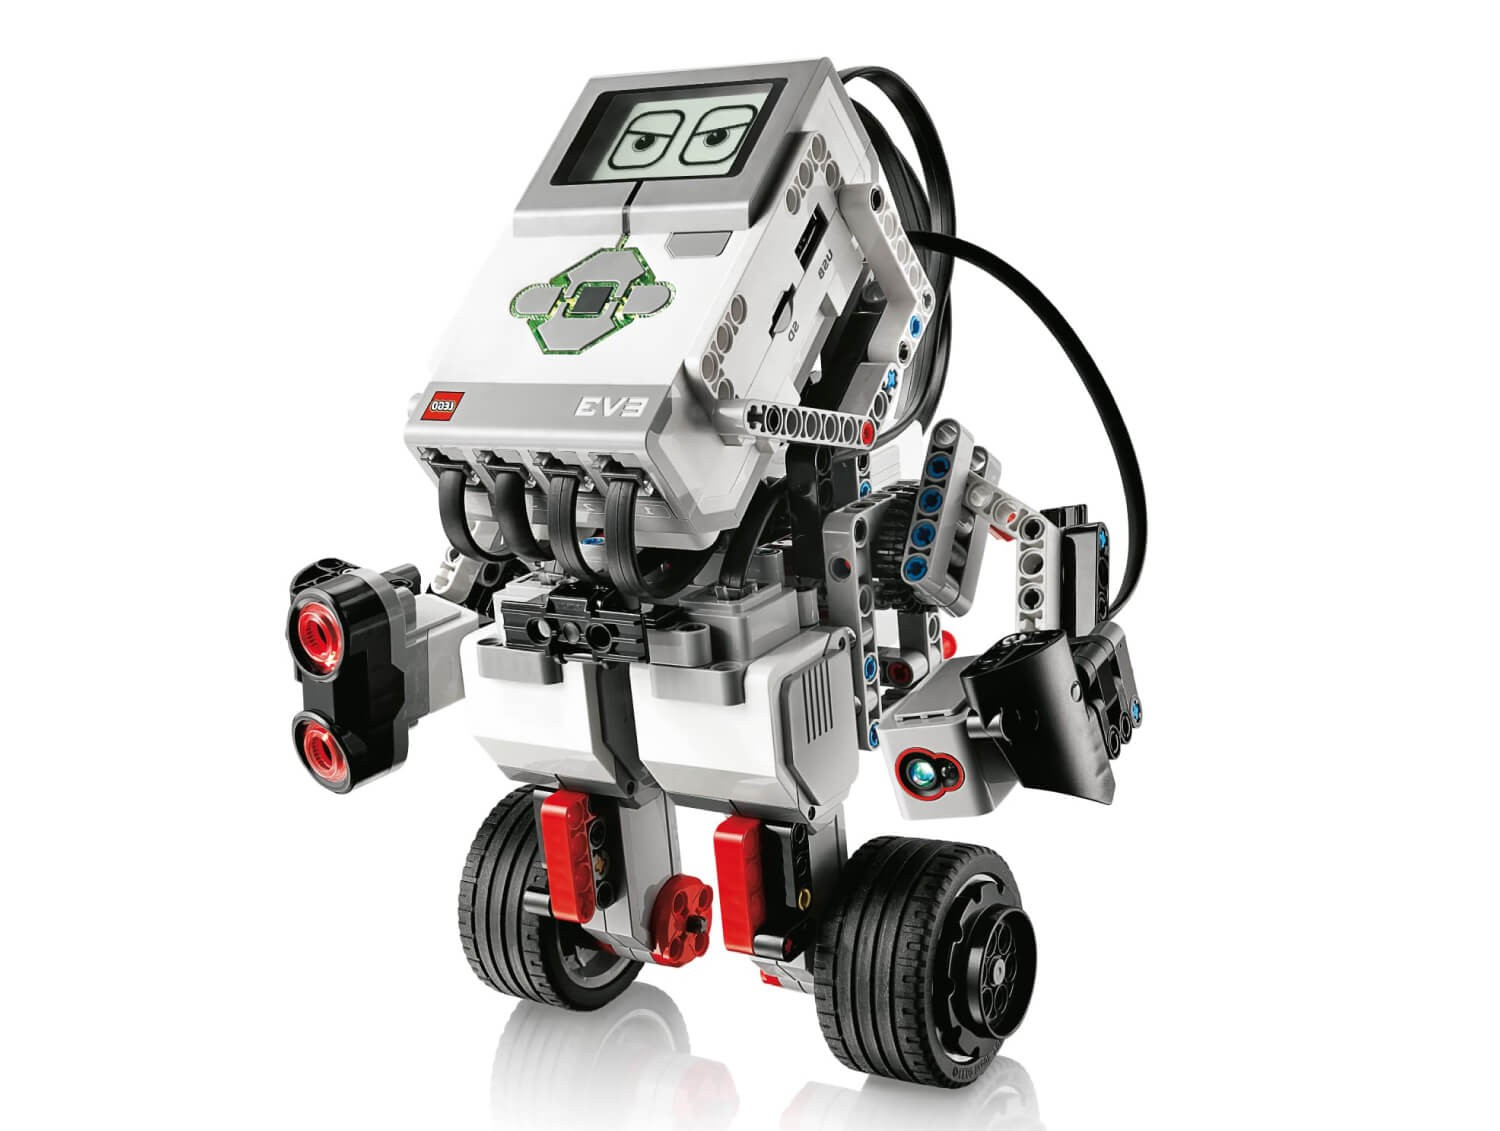
\includegraphics[width=0.4\textwidth]{img/legomind.jpg}
        \caption{Ejemplo de \textit{robot} montado con \textit{Mindstorms}} \label{fig:lego}
    \end{figure}
    \item \textit{\textbf{Makeblock}}\cite{bib:makeblock}: plataforma de construcción robótica muy accesible que permite la creación de \textit{robots} con \textit{kits} dirigidos a todo tipo de público. El \textit{robot} que se construye con estos \textit{kits} es el \textit{mBot}:
        \begin{figure}[H]
        \centering
        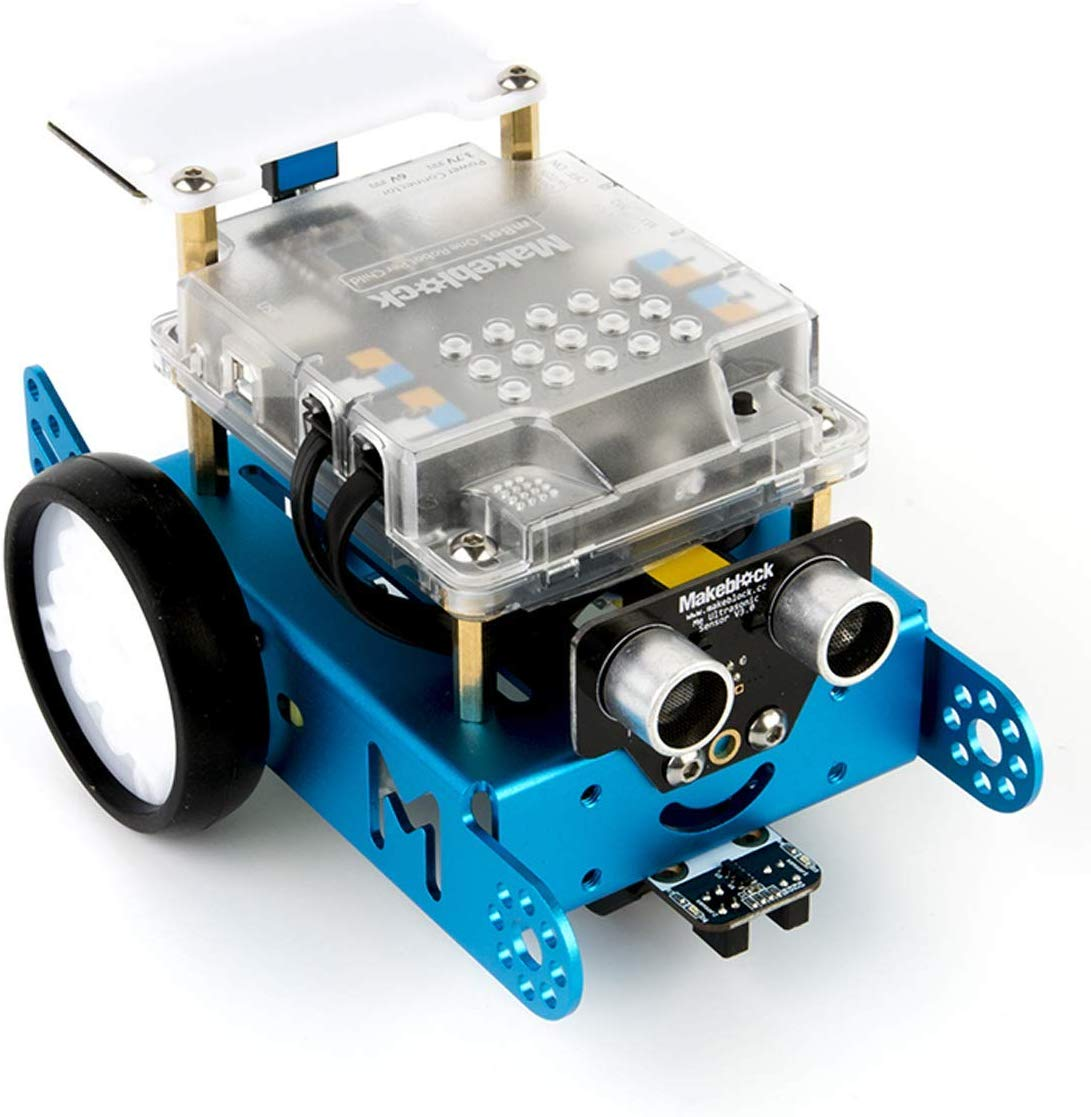
\includegraphics[width=0.3\textwidth]{img/mBotReal.jpg}
        \caption{mBot de la plataforma \textit{Makeblock}} \label{fig:makeblock}
    \end{figure}

    \item \textit{\textbf{Arduino}}\cite{bib:arduino}: Plataforma de creación electrónica. Permite crear microordenadores a los que dar multitud de usos con una sola placa, que dispone de entradas para periféricos y un microcontrolador.

\end{itemize}{}
